\section*{Описание алгоритма}

При арифметическом кодировании для кодируемой последовательности 
создается уникальный идентификатор или тег. Этот тег соответствует
двоичной дроби, которая становится двоичным кодом последовательности.
Уникальный арифметический код может быть сгенерирован для
последовательности длиной $m$ без необходимости генерировать кодовые
слова для всех последовательностей длины $m$. Это не похоже на ситуацию
с кодами Хаффмана. Чтобы сгенерировать код Хаффмана для
последовательности длины $m$, где код не является конкатенацией кодовых
слов для отдельных символов, нам необходимо получить коды Хаффмана для
всех последовательностей длины $m$.

Чтобы отличить последовательность символов от другой последовательности
символов, нам нужно пометить ее уникальным идентификатором. Один из
возможных наборов тегов для представления последовательностей символов -
это числа в единичном интервале $[0,1)$. Поскольку количество чисел в
единичном интервале бесконечно, должно быть возможно присвоить
уникальный тег каждой отдельной последовательности символов.

Процедура создания тега работает за счет уменьшения размера интервала,
в котором находится тег, по мере получения все большего количества
элементов последовательности.

\pagebreak

\subsection*{Пример}

Рассмотрим трехбуквенный алфавит $A = \{a_1, a_2, a_3\}$ с 
$P(a_1) = 0{,}7$, $P(a_2) = 0{,}1$ и $P (a_3) = 0{,}2$.
Используя отображение $F_X (1) = 0{,}7$, $F_X (2) = 0{,}8$ и
$F_X (3) = 1$ разбиваем единичный интервал, как показано на рисунке
ниже.
\begin{center}
    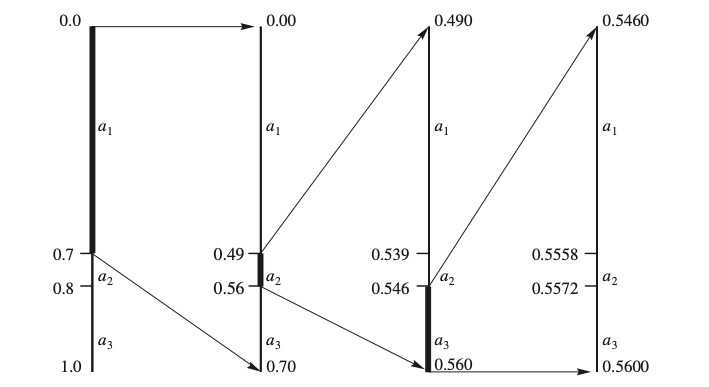
\includegraphics[scale=0.5]{src/1.png}
\end{center}
Для последовательности, начинающейся с $a_1, a_2, a_3,\dots$, к тому
времени, когда будет получен третий символ $a_3$, тег будет ограничен
субынтервалом $[0,546, 0,56)$. Если бы третьим символом был $a_1$ вместо
$a_3$, тег находился бы в подынтервале $[0,49, 0,539)$, который не
пересекается с подынтервалом $[0,546, 0,56)$. Даже если с этого момента
две последовательности идентичны (одна начинается с $a_1$, $a_2$, $a_3$, а
другая начинается с $a_1$, $a_2$, $a_1$), интервал тегов для двух
последовательностей всегда будет непересекающимся.

\pagebreak